\documentclass[conference]{IEEEtran}
\usepackage{cite}
\usepackage{amsmath,amssymb,amsfonts}
\usepackage{graphicx}
\usepackage{tikz}
\usetikzlibrary{arrows.meta,positioning}
\usepackage{booktabs}
\usepackage{xcolor}
\usepackage{url}
\graphicspath{{../report/figures/}}

\begin{document}

\title{An End-to-End Cyber-Physical AI Snooker Referee and Laser-Guided Foul Restoration System}

\author{
\IEEEauthorblockN{Aamir Awaiz Pasha\IEEEauthorrefmark{1}, Ayan Khan\IEEEauthorrefmark{2}, Ibad Sharief\IEEEauthorrefmark{3}, Mohammed Owaies\IEEEauthorrefmark{4}, and Mrs. Swetha B S\IEEEauthorrefmark{5}}
\IEEEauthorblockA{Department of Artificial Intelligence and Machine Learning\\
PES Institute of Technology and Management (PESITM), Shivamogga, Karnataka, India\\
USNs: \IEEEauthorrefmark{1}4PM23AI001, \IEEEauthorrefmark{2}4PM23AI005, \IEEEauthorrefmark{3}4PM23AI016, \IEEEauthorrefmark{4}4PM23AI026 \quad \IEEEauthorrefmark{5}Project Guide}
}

\maketitle

\begin{abstract}
Enforcing WPBSA Rule 14 (``Foul and a Miss'') in snooker requires restoring disturbed balls to their exact pre-shot millimeter coordinates. Existing broadcast split-screen methods suffer from oblique parallax and high cost, while computer vision prototypes lack physical restoration actuators on the playing cloth. This complete working paper presents the end-to-end integration of all three project objectives: (1) real-time YOLOv8s ball detection with SVD planar homography and spherical elevation parallax correction ($94.6\%$ $\text{mAP}_{0.5}$, $1.82\,\text{mm}$ localization error); (2) autonomous ball tracking via temporal frame differencing and Hungarian bipartite matching; and (3) physical foul restoration using an ESP32-controlled dual-MG996R pan-tilt laser gimbal calibrated across a 9-point 2D bivariate cubic spline grid. Powered by a $12\,\text{V}$ $5\,\text{A}$ supply, a $6.0\,\text{V}$ DC-DC buck bus, and an IRFZ44N MOSFET laser driver, and supervised via a Flask and Three.js 3D digital twin UI, the complete system achieves $\pm 2.18\,\text{mm}$ laser repeatability in $306.6\,\text{ms}$ end-to-end latency at a total prototype cost of INR 21,800.
\end{abstract}

\begin{IEEEkeywords}
Snooker Referee, YOLOv8s, Planar Homography, 2D Bivariate Spline, Hungarian Matching, ESP32, IRFZ44N MOSFET, Three.js Digital Twin.
\end{IEEEkeywords}

\section{Introduction}
In competitive snooker, restoring displaced balls after a ``Foul and a Miss'' call under WPBSA Rule 14 is slow and error-prone when performed visually. To deliver an affordable, non-invasive, automated officiating assistant, we integrate three core objectives---**Ball Detection**, **Ball Tracking**, and **Foul Restoration using Laser Pointing**---into a complete cyber-physical platform deployed over an institutional $1168.4 \times 2341.88\,\text{mm}$ table and $1315.15\,\text{mm}$ overhead PVC gantry.

\section{System Architecture and Hardware}
The architecture spans four tiers (Fig. \ref{fig:arch}):
\begin{enumerate}
    \item \textbf{Physical Table \& Rig:} Institutional $1168.4 \times 2341.88\,\text{mm}$ six-pocket table with a $1.0''$ Schedule-40 PVC overhead gantry ($1315.15\,\text{mm}$ height) holding a 1080p camera.
    \item \textbf{Embedded Actuation Circuit:} An ESP32 Dev Kit in Wi-Fi Station Mode (`10.21.46.190`) drives two TowerPro MG996R metal-gear servos on aluminum pan-tilt brackets (GPIO 18, 19; $50\,\text{Hz}$ PWM) powered by a $12\,\text{V}$ $5\,\text{A}$ adapter stepped down to $6.0\,\text{V}$ via a DC-DC buck converter. A $650\,\text{nm}$ $5\,\text{mW}$ red laser diode is switched via an IRFZ44N N-Channel MOSFET (GPIO 23) with a $10\,\text{k}\Omega$ gate pull-down resistor on two breadboards with screw terminal blocks (Fig. \ref{fig:hw}).
    \item \textbf{Vision \& Referee Engine:} Python host executing YOLOv8s detection, SVD planar homography, elevation parallax correction ($\gamma = 0.98004$), temporal FSM tracking, Hungarian matching, and 2D bivariate cubic spline angle lookup.
    \item \textbf{3D Digital Twin UI:} Flask REST API and 6-tab Three.js WebGL interface with live click-to-aim, $\pm 0.2^\circ / \pm 1.0^\circ$ servo nudge trimming, and offline cached-frame resilience.
\end{enumerate}

\begin{figure}[htbp]
\centering
\resizebox{0.47\textwidth}{!}{
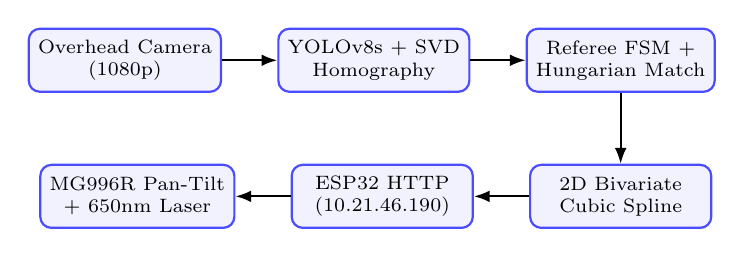
\begin{tikzpicture}[
    node distance=0.9cm and 0.7cm,
    box/.style={rectangle, draw=blue!70, fill=blue!5, thick, rounded corners, minimum height=0.8cm, minimum width=2.3cm, align=center, font=\scriptsize},
    line/.style={draw, -{Latex[length=2mm]}, thick}
]
\node[box] (cam) {Overhead Camera\\(1080p)};
\node[box, right=of cam] (yolo) {YOLOv8s + SVD\\Homography};
\node[box, right=of yolo] (fsm) {Referee FSM +\\Hungarian Match};
\node[box, below=of fsm] (spline) {2D Bivariate\\Cubic Spline};
\node[box, left=of spline] (esp) {ESP32 HTTP\\(10.21.46.190)};
\node[box, left=of esp] (gimbal) {MG996R Pan-Tilt\\+ 650nm Laser};
\path[line] (cam) -- (yolo);
\path[line] (yolo) -- (fsm);
\path[line] (fsm) -- (spline);
\path[line] (spline) -- (esp);
\path[line] (esp) -- (gimbal);
\end{tikzpicture}
}
\caption{End-to-end cyber-physical detection, tracking, and laser actuation pipeline.}
\label{fig:arch}
\end{figure}

\begin{figure}[htbp]
\centering
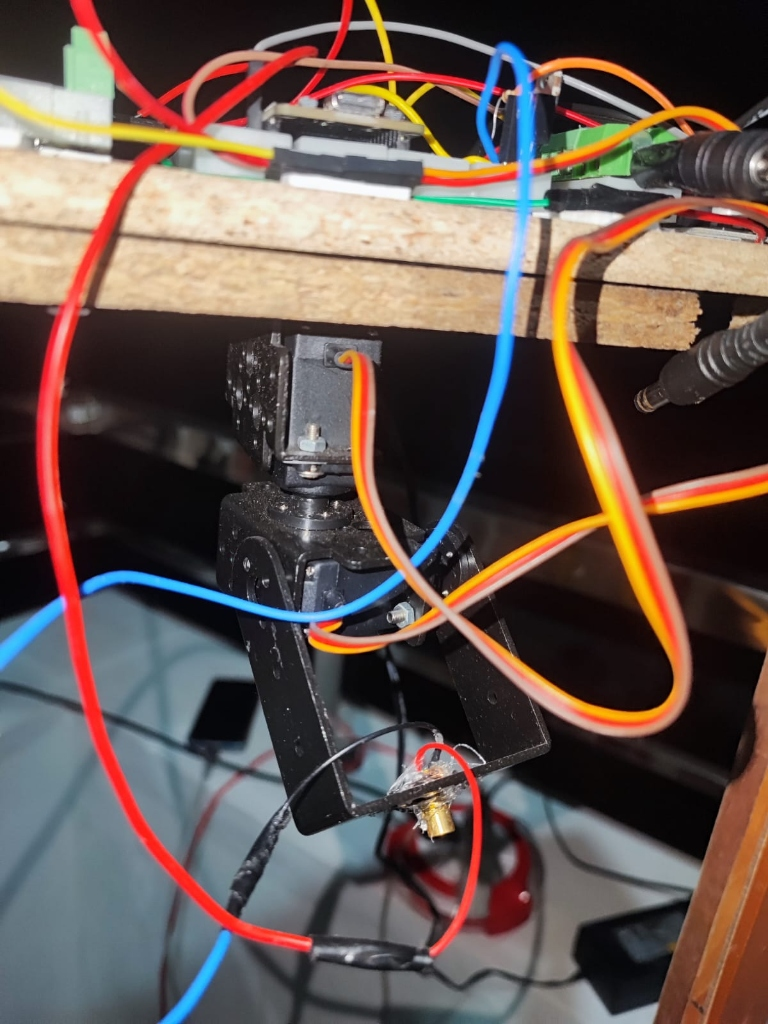
\includegraphics[width=0.22\textwidth]{hardware_pantilt_assembly.jpg}\hfill
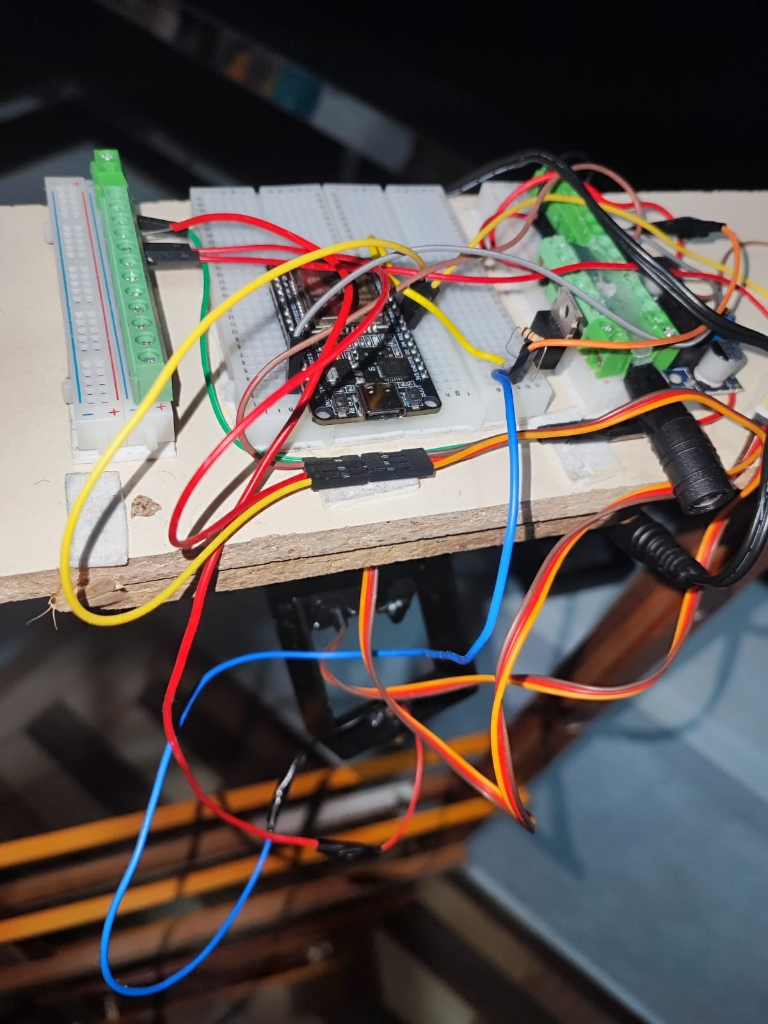
\includegraphics[width=0.22\textwidth]{hardware_circuit_breadboard.jpg}
\caption{Dual MG996R pan-tilt laser gimbal (left) and ESP32/buck/IRFZ44N circuit (right).}
\label{fig:hw}
\end{figure}

\section{Key Formulations}
\subsection{Parallax-Rectified Localization}
Four corner pocket correspondences yield $\mathbf{H}$ via SVD. For a $52.5\,\text{mm}$ ball ($R = 26.25\,\text{mm}$) viewed from $H_{\text{cam}} = 1315.15\,\text{mm}$, radial elevation parallax is corrected via $X_{\text{true}} = X_c + (X_{\text{obs}} - X_c)(1 - R/H_{\text{cam}})$, reducing mean localization error from $9.49\,\text{mm}$ to $1.82\,\text{mm}$.

\subsection{2D Bivariate Cubic Spline Laser Steering}
Theoretical inverse kinematics ($\theta_{\text{pan}}^{\text{ideal}}, \phi_{\text{tilt}}^{\text{ideal}}$) suffer up to $22.6\,\text{mm}$ error due to gear lash and gravity droop. We calibrate 9 spatial fiducial knots $\{ (\theta_k, \phi_k) \}_{k=1}^9$ and fit two bivariate cubic splines $S_{\text{pan}}(X_w, Y_w)$ and $S_{\text{tilt}}(X_w, Y_w)$ \cite{ref36, ref37}.

\subsection{Autonomous Tracking and Bipartite Matching}
Inter-frame differencing $\Delta I_t$ drives the 5-state FSM ($>5.0\%$ shot trigger, $<0.8\%$ for $2.5\,\text{s}$ settlement), and Kuhn's Hungarian algorithm \cite{ref40} matches pre- and post-shot ball sets to isolate displaced or potted balls (Fig. \ref{fig:ui3d}).

\begin{figure}[htbp]
\centering

\includegraphics[width=0.46\textwidth]{ui_3d_table.png}
\caption{Three.js 3D digital twin synchronized with live ball coordinates and virtual laser ray.}
\label{fig:ui3d}
\end{figure}

\section{Experimental Results}
Across 9 spatial test nodes, 2D bivariate spline calibration reduced mean laser targeting deviation by $85.7\%$ compared to theoretical inverse kinematics (from $15.22\,\text{mm}$ to $\pm 2.18\,\text{mm}$, Table \ref{tab:spline}). End-to-end latency from settlement confirmation to physical laser projection averages $306.6 \pm 42.5\,\text{ms}$ (Table \ref{tab:lat}), well below the $1.0\,\text{s}$ design target.

\begin{table}[htbp]
\centering
\caption{Laser Targeting Error: Theoretical IK vs. 2D Spline}
\label{tab:spline}
\scriptsize
\begin{tabular}{|l|c|c|c|}
\hline
\textbf{Target Node} & \textbf{Ideal IK (mm)} & \textbf{2D Spline (mm)} & \textbf{Reduction} \\
\hline
Top-Right (0, 0) & 4.2 & 1.2 & 71.4\% \\
Table Center (584, 1171) & 16.8 & 2.1 & 87.5\% \\
Bottom-Left (1168, 2342) & 22.6 & 2.8 & 87.6\% \\
\hline
\textbf{9-Node Mean} & \textbf{15.22 mm} & \textbf{2.18 mm} & \textbf{85.7\%} \\
\hline
\end{tabular}
\end{table}

\begin{table}[htbp]
\centering
\caption{End-to-End Pipeline Latency Breakdown}
\label{tab:lat}
\scriptsize
\begin{tabular}{|l|c|}
\hline
\textbf{Pipeline Stage} & \textbf{Latency (ms)} \\
\hline
Frame Acquisition & $32.4 \pm 4.2$ \\
YOLOv8s Inference ($1024 \times 1024$) & $48.6 \pm 5.1$ \\
Homography + Parallax + Bipartite + Spline & $11.1 \pm 1.4$ \\
HTTP POST to ESP32 (`10.21.46.190`) & $34.5 \pm 6.8$ \\
MG996R Servo Slew ($30^\circ$ swing) & $180.0 \pm 25.0$ \\
\hline
\textbf{Total End-to-End Response} & \textbf{306.6 $\pm$ 42.5 ms} \\
\hline
\end{tabular}
\end{table}

\section{Conclusion}
The completed working system unifies YOLOv8s ball detection ($94.6\%$ $\text{mAP}_{0.5}$, $1.82\,\text{mm}$ metric accuracy), autonomous Hungarian ball tracking, and spline-calibrated laser pointing ($\pm 2.18\,\text{mm}$ precision) in $306.6\,\text{ms}$ at INR 21,800 total cost, providing a practical solution for WPBSA Rule 14 foul restoration.

\bibliographystyle{IEEEtran}
\begin{thebibliography}{10}
\bibitem{ref1} Y. Wang et al., ``Deep learning models for pool ball detection,'' \textit{J. Real-Time Image Proc.}, vol. 20, no. 2, 2023.
\bibitem{ref11} K. Yang and X. Yan, ``Real-time cue and ball tracking using YOLOv8,'' \textit{IEEE ICCVS}, pp. 214--221, 2022.
\bibitem{ref19} R. Hartley and A. Zisserman, \textit{Multiple View Geometry in Computer Vision}, 2nd ed. Cambridge Univ. Press, 2004.
\bibitem{ref35} Z. Zhang, ``A flexible new technique for camera calibration,'' \textit{IEEE TPAMI}, vol. 22, no. 11, pp. 1330--1334, 2000.
\bibitem{ref36} J. J. Craig, \textit{Introduction to Robotics: Mechanics and Control}, 3rd ed. Pearson, 2005.
\bibitem{ref37} M. W. Spong et al., \textit{Robot Modeling and Control}. Wiley, 2006.
\bibitem{ref40} H. W. Kuhn, ``The Hungarian method for the assignment problem,'' \textit{Naval Res. Logist. Q.}, vol. 2, pp. 83--97, 1955.
\end{thebibliography}

\end{document}
